\documentclass{beamer}

\usetheme{Madrid}

\title[Smart Share]{Smart Share}
\author[Blazanome]{Romain Benoît, Théo Choné, Ewan Chorynski, Florian Delhon, Théo Gaigé, Amar Hasan Tawfiq, Alix Peigue}
\institute[INSA Lyon]{INSA Lyon}
\date{2024}

\usepackage[T1]{fontenc}
\usepackage[utf8]{inputenc}
\usepackage{listings}
\usepackage{tikz}
\usepackage{xcolor}
\usetikzlibrary{positioning}
\usetikzlibrary{shapes.geometric}

\lstset{%
basicstyle=\tiny\ttfamily,
breaklines = true,
language=C,
numbers=left,
numberstyle=\tiny\color{gray},
keywordstyle=\color{blue}\ttfamily,
stringstyle=\color{red}\ttfamily,
commentstyle=\color{green}\ttfamily,
morecomment=[l][\color{magenta}]{\#},
xleftmargin=2em,frame=single,framexleftmargin=1.5em
}

\newcommand*{\thead}[1]{\multicolumn{1}{|c|}{\bfseries #1}}
\newcommand*{\local}[1]{\lstinline|\_#1|}

\begin{document}

\frame{\titlepage}

\begin{frame}
    \frametitle{Objectifs}
    \begin{block}{Existant}
        \begin{itemize}
            \item Google Docs: édition sur le navigateur, serveurs propriétaires de Google
            \item LiveShare: restreint à VSCode
            \item CodeTogether: payant, propriétaire
        \end{itemize}
        Ces solutions sont restrictives ou demandent à utiliser une nouvel outil d'édition ou sont payantes.
        On doit pouvoir améliorer cela !
    \end{block}
    \begin{block}{Notre proposition}
        Une solution open-source d'édition de fichiers simultanée fonctionnant sur plusieurs éditeurs.
        \begin{itemize}
            \item Un protocole de communication
            \item Un client exécutable universel à tous les éditeurs de textheight
            \item Une intégration simple dans les éditeurs/IDE
        \end{itemize}
    \end{block}
\end{frame}

\begin{frame}
    \frametitle{Objectifs}
    \begin{block}{Temps réel}
        \begin{itemize}
            \item Latence faible
            \item Edition simultanée des fichiers (nombreux enjeux abordés en détail dans les slides suivantes)
        \end{itemize}
    \end{block}
    \begin{block}{Interopérabilité}
        \begin{itemize}
            \item Fonctionalités équivalentes sur plusieurs éditeurs
            \item Ajout communautaire d'éditeurs
            \item Facilité d'intégration
        \end{itemize}
    \end{block}
\end{frame}

\section{Première itération}
\begin{frame}
    \frametitle{Architecture globale}
    \includegraphics[width=\textwidth,height=0.8\textheight,keepaspectratio]{archi.png}
\end{frame}

\begin{frame}
    \frametitle{Architecture globale}

    \begin{block}{Avantages}
        \begin{itemize}
            \item Factoriser la complexité dans le client
            \item Favoriser l'interopérabilité
            \item Faciliter la communication avec le serevur
       \end{itemize}
    \end{block}

    \begin{block}{Inconvénients}
        \begin{itemize}
            \item Deux protocoles à gérer
            \item Deux points de synchronisation
            \item Toujours un peu de logique à coder directement dans l'IDE
        \end{itemize}
    \end{block}
\end{frame}

\begin{frame}
    \frametitle{Choix du langage}
    \framesubtitle{Rust}

    \begin{columns}
        \begin{column}{0.7\textwidth}
            \begin{itemize}
                \item \textit{Fast, Reliable, Productive. Pick Three.}
                \item \textit{Fearless parallelism}
                \item Langage de programmation système
                \item Adapté à la programmation parallèle sans risque
                \item Grand entrain de la part du groupe pour apprendre ce nouveau langage
            \end{itemize}
        \end{column}
        \begin{column}{0.3\textwidth}
            \includegraphics[width=\textwidth,height=0.2\textheight,keepaspectratio]{ferris.png}
        \end{column}
    \end{columns}
\end{frame}
\begin{frame}[fragile]
    \frametitle{Transport de données}
    \framesubtitle{Sérialisation}
    \begin{block}{Sur la ligne}
        \begin{itemize}
            \item Messages sérialisés en JSON
            \item Un message par ligne
        \end{itemize}
    \end{block}
    \begin{exampleblock}{Exemple}
        \begin{lstlisting}
{"action":"update","changes":[{"offset":3413,"delete":0,"text":"i"}]}
{"action":"update","changes":[{"offset":3414,"delete":2,"text":""}]}
{"action":"update","changes":[{"offset":3436,"delete":0,"text":"lstlisting"}]}
{"action":"ack"}
        \end{lstlisting}
    \end{exampleblock}
    \begin{block}{Côté Rust}
        \begin{itemize}
            \item Structures fortement typés
            \item Des Streams pour recevoir
            \item Des Sinks pour envoyer Un message par ligne
        \end{itemize}
    \end{block}
\end{frame}

\begin{frame}
    \frametitle{Solution naïve}

    \begin{block}{Serveur}
        \begin{itemize}
            \item Transmet les changements reçus d'un client vers tous les autres
            \item Ressemble à un simple chat
        \end{itemize}
    \end{block}
    \begin{block}{Client}
        \begin{itemize}
            \item Transmet simplement les messages entre l'IDE et le serveur
            \item Simple boîte au lettre
        \end{itemize}
    \end{block}
    \begin{alertblock}{Ce n'est pas si simple !}
        Gros problèmes lorsque plusieurs personnes écrivent en même temps.
    \end{alertblock}
\end{frame}

\begin{frame}
    \frametitle{Operational Transform (OT) - 1/3}
    \begin{block}{Contexte}
        \begin{itemize}
            \item $\neq$ Git - changements asynchrones $\Rightarrow$ nécessité de \textit{commit}
            \item Google Docs, Etherpad, LiveShare - changements synchrones, temps-réel
            \item Deux stratégies - \textit{Event passing} ou \textit{Differential sync}
        \end{itemize}
    \end{block}

    \begin{block}{Principe}
        \begin{itemize}
            \item Algorithme de type \textit{Event passing}
            \item Chaque client envoie les \textit{events} caractère par caractère au serveur
            \item (Exemples : 'M' inséré à la position 4, suppression d'un caractère à partir de la position 10, ...)
            \item Objectif : maintenir et synchroniser un état cohérent entre les utilisateurs
        \end{itemize}
    \end{block}
\end{frame}

\begin{frame}
    \frametitle{Operational Transform (OT) - 2/3}
    \begin{block}{Problème}
        \begin{itemize}
            \item Si tous les clients exécutent les mêmes \textit{events} dans un ordre différent
            \item $\Rightarrow$ résultats potentiellement différents
            \item Exemple : $a = ins(X, 1)$ et $b = ins(Y, 1) \Rightarrow a \times b \neq b \times a$
        \end{itemize}
    \end{block}

    \begin{block}{Solution : Transformation}
        \begin{columns}
            \begin{column}{0.3\textwidth}
                \includegraphics[width=\textwidth,height=0.8\textheight,keepaspectratio]{../images/diamond_ot.png}
            \end{column}
            
            \begin{column}{0.7\textwidth}
                \begin{itemize}
                    \item Fonction de transformation - calculer les nouvelles opérations complémentaires tel que :
                    \item $\Rightarrow$ $a \times b' = b \times a'$
                    \item Exemple - $a = ins(X, 1)$ et $b = ins(Y, 1) \Rightarrow a' = a$ et $b' = ins(Y, 2)$
                \end{itemize}
            \end{column}
        \end{columns}
    \end{block}
    
    $\Rightarrow$ \textit{Crate} Rust "operational\_transform" et structure OperationSeq

\end{frame}

\begin{frame}
    \frametitle{Operational Transform (OT) - 3/3}
    \begin{block}{Application dans SmartShare}
        \begin{itemize}
            \item Décomposition du document en trois ensembles : $A \times X \times Y$
            \item $A$ : état stable, $X$ : changements envoyés, $Y$ : changements non envoyés
            \item Gestion des conflits dans le Client et le Serveur
        \end{itemize}
    \end{block}

    \begin{block}{Serveur}
        \begin{itemize}
            \item Approbation des changements envoyés par le Client
            \item Calcul des nouvelles opérations pour maj du doc Serveur + envoi aux Clients
        \end{itemize}
    \end{block}

    \begin{block}{Client}
        \begin{itemize}
            \item Enregistrement des changements locaux IDE
            \item Soumission de ses changements au Serveur
            \item Application des changements des autres Clients
        \end{itemize}
    \end{block}
\end{frame}

\begin{frame}
    \frametitle{Plugins IDE}
    \begin{block}{Fonctionnalités}
        \begin{itemize}
            \item Deux plugins IDE développés : l'un pour Neovim en Lua, l'autre pour VSCode en TypeScript
            \item Un ensemble de fonctionnalités communes : édition de fichier simultanée en temps réel avec des curseurs
            \item Les plugins IDE communiquent avec le client dans l'architecture globale
        \end{itemize}
    \end{block}
\end{frame}

\begin{frame}
    \frametitle{Protocole 1/4 - Initialisation}
    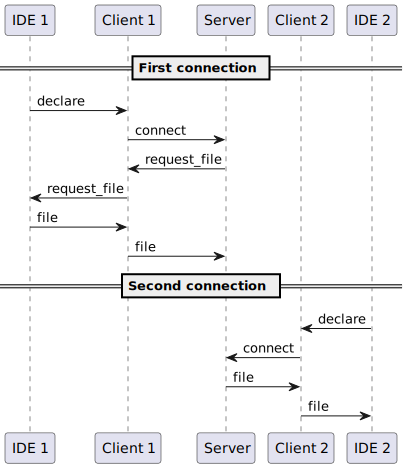
\includegraphics[width=\textwidth,height=0.8\textheight,keepaspectratio]{diagrams/1.png}
\end{frame}

\begin{frame}
    \frametitle{Protocole 2/4 - Modification}
    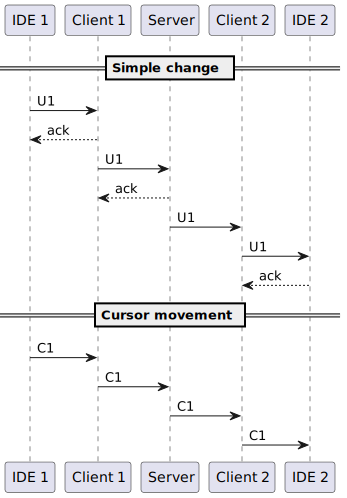
\includegraphics[width=\textwidth,height=0.8\textheight,keepaspectratio]{diagrams/2.png}
\end{frame}

\begin{frame}
    \frametitle{Protocole 3/4 - Conflit client-serveur}
    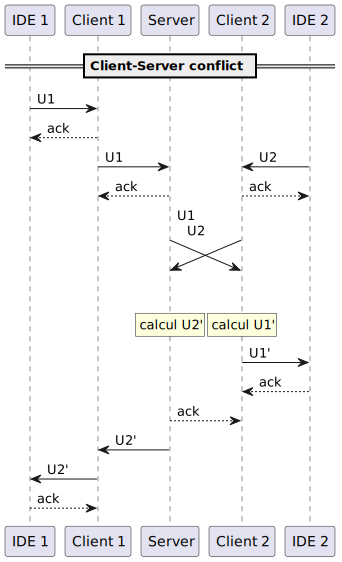
\includegraphics[width=\textwidth,height=0.8\textheight,keepaspectratio]{diagrams/3.png}
\end{frame}

\begin{frame}
    \frametitle{Protocole 4/4 - Conflit IDE-client}
    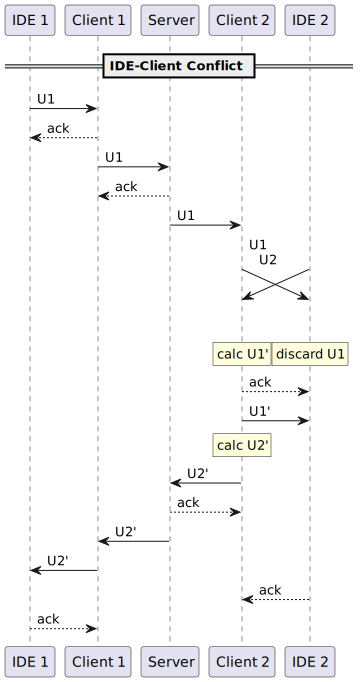
\includegraphics[width=\textwidth,height=0.8\textheight,keepaspectratio]{diagrams/4.png}
\end{frame}

\begin{frame}
    \frametitle{Plugins IDE}
    \framesubtitle{Neovim}
    \begin{block}{Configuration}
        \begin{itemize}
            \item Comme pour tout plugin, on doit require('smartshare') dans la config Neovim
            \item Se lance avec la commande :SmartShareConnect <ip\_serveur>
            \item Cette commande aura pour effet de lancer automatiquement le client
        \end{itemize}
    \end{block}
\end{frame}

\begin{frame}
    \frametitle{Plugins IDE}
    \framesubtitle{Neovim}
    \begin{block}{Utilisation}
        \begin{itemize}
            \item Après que le client se soit connecté au serveur, il récupère le fichier suivi ou il upload son propre fichier s'il est le premier
            \item L'utilisateur peut ainsi modifier le fichier, voir les modifications des autres et voir leurs curseurs
        \end{itemize}
    \end{block}
\end{frame}

\begin{frame}
    \frametitle{Plugins IDE}
    \framesubtitle{Neovim}
    \begin{block}{Fonctionnement}
        \begin{itemize}
            \item Utilisation de l'api Neovim et des builtins Vim (nvim\_buf\_attach, callback on\_bytes...)
            \item Communication avec le client par stdin et stdout au format json
            \item Manipulation du texte en octets (nvim\_buf\_get\_text, nvim\_buf\_set\_text...)
            \item Utilisation d'extmarks pour les curseurs (on highlight les cellules du terminal)
        \end{itemize}
    \end{block}
\end{frame}

\begin{frame}
    \frametitle{Chars vs octets}
    \framesubtitle{Des encodages et des formats d'édition différents}
    \begin{block}{Problème}
        \begin{itemize}
            \item Il n'y a pas qu'ASCII : différents encodages comme UTF-8 qui ont des caractères plus grands qu'un octet
            \item Les IDE permettent aux plugins de manipuler le texte de différentes manières : caractères, octets, lignes/colonnes...
            \item Notre bibliothèque OT utilise des caractères, et cela fait plus sens pour du texte : on convertit donc tout en caractères
            \item Les offsets de fichier et les delete sont convertis vers des offsets de chars grâce à des byte slices
            \item Le client est lancé avec l'option "--format <bytes/chars>" afin de lui notifier le format utilisé par le plugin
        \end{itemize}
    \end{block}
\end{frame}

\begin{frame}
    \frametitle{Gestion de projet}
    \framesubtitle{Méthode agile}
    \begin{block}{Organisation générale}
        \begin{itemize}
            \item Projet séparés en tâches : plugins IDE, serveur \& client, gestion de conflits, protocoles de communication, ...
            \item 1 sprint par jour avec état d'avancement chaque matin
            \item Document de suivi décrivant les objectifs du jour
            \item Objectif d'avoir toujours une version fonctionnelle : d'abord envoyer un simple char, puis plusieurs, puis gérer les conflits, ...
        \end{itemize}
    \end{block}
    \pause
    \begin{exampleblock}{Exemple}
        Cette stratégie nous a permis d'écarter la piste de Kyte au profit d'EasySync assez rapidement
    \end{exampleblock}
\end{frame}

\begin{frame}
    \frametitle{Conclusion}
    \framesubtitle{Bilan du projet}
    \begin{block}{Fonctionnalités non développées}
        \begin{itemize}
            \item Utilisation en réseau non local
            \item Partage de plusieurs fichiers en même temps
            \item Support d'autres éditeurs de texte
        \end{itemize}
    \end{block}
    \pause
    \begin{block}{Fonctionnalités développées}
        \begin{itemize}
            \item Support de plusieurs IDE sur le même fichier
            \item Synchronisation en temps réel
            \item Gestion des conflits
            \item Visualisation des curseurs
        \end{itemize}
    \end{block}
    \pause
    \begin{exampleblock}{Belle récompense}
        Cette présentation a été codée à plusieurs, simultanément, en utilisant Smart Share !
    \end{exampleblock}
\end{frame}

\end{document}

 
